% ncse_new/\problems/ch_piecewisepolynomials/ex_CubicSplines.tex
%  solution:  ex_CubicSpline.m  ex_CubicSpline.eps

\begin{problem}[Cubic Splines \coreproblem] \label{prb:CubicSplines}
  Since they mimic the behavior of an elastic rod pinned at fixed points, see
  \lref{rem:csrod}, cubic splines are very popular for creating ``aesthetically
  pleasing'' interpolating functions. However, in this problem we look at a
  cubic spline from the perspective of its defining properties, see
  \lref{def:spline}, in order to become more familiar with the concept of
  spline function and the consequences of the smoothness required %stipulated
  by the definition.

 For parameters $\alpha,\beta\in\bbR$ we define the function
  $s_{\alpha,\beta}:[-1,2]\to \bbR$ by
  \begin{gather}    \label{eq:ex_CubicSplines}
    s_{\alpha,\beta}(x) = \left\{\begin{array}{ll}
        (x+1)^4+\alpha(x-1)^4+1 & x\in[-1,0]\\
        -x^3-8\alpha x +1 &       x\in(0,1]\\
        \beta x^3+8x^2 + \frac{11}{3} & x\in(1,2]
      \end{array}\right.
  \end{gather}


% interesting alternative choice!!!
% define s(x) = x^3+x^2+6+\beta(x-1)^2   in the 3rd interval
% it is C^1 for every beta, C^2 only for beta = -7
% they can play with the plot and see 2nd derivatives as curvature
% matlab line:   y3 = x3.^3 + x3.^2 + 6 + beta*( x3-1 ).^2;


%=====================================================================================================
\begin{subproblem}[2] \label{subprb:CubicSplines_1}     % a
    Determine $\alpha,\beta$ such that $s_{\alpha,\beta}$ is a cubic spline in $\Cs_{3,M}$
    with respect to the node set $M=\{-1,0,1,2\}$.
    Verify that you actually obtain a cubic spline.

    %\Hint: The continuity conditions for $s$, $s'$, and $s''$ have to hold at internal nodes.

\begin{solution}
We immediately see that $\alpha=-1$ is necessary to get a polynomial of $3^{\text{rd}}$ degree.

Furthermore, from the condition
$$8=s_{-1,\beta}(1^-)=s_{-1,\beta}(1^+)=\beta+8+\frac{11}{3}\qquad
\text{we get }\quad\beta=-\frac{11}{3}.$$
It remains to check the continuity of $s,s',s''$ in the nodes $0$ and $1$. Indeed, we have
$$s_{-1,\beta}'(x)=
\begin{cases}
4(x+1)^3+4\alpha(x-1)^3   \\
-3x^2-8\alpha             \\
3\beta x^2+16x
\end{cases}
s_{-1,\beta}''(x)
\begin{cases}
 12(x+1)^2+12\alpha(x-1)^2  &-1\le x\le0,\\
 -6x  & 0<x\le 1,\\
6\beta x+16 & 1<x<2.
\end{cases}$$
Therefore the values in the nodes are

\begin{tabular}{  c | c c | c c | }%\hline
 & $0^-$ & $0^+$ & $1-$ & $1^+$\\ \hline
$s$ & $2+\alpha$ & 1 & $-8\alpha$ & $\beta+8+11/3$\\
$s'$ & $4-4\alpha$ & $-8\alpha$ & $-3-8\alpha$ & $3\beta+16$\\
$s''$ & $12+12\alpha$ & 0 & -6 & $6\beta+16$%\\ \hline
\end{tabular}
$\begin{matrix}
\alpha=-1, \\ \beta=-11/3\rightarrow
\end{matrix}$
\begin{tabular}{  c | c c | c c | }%\hline
 & $0^-$ & $0^+$ & $1-$ & $1^+$\\ \hline
$s$ & 1 & 1 & 8 & 8\\
$s'$ & 8 & 8 & 5 & 5\\
$s''$ & 0 & 0 & -6 & -6%\\ \hline
\end{tabular}

They agree for our choice of the parameters.
% \[ \begin{array}{rclrcl}
% s_{\alpha,\beta}(0^-)&=&2+\alpha=1 & s_{\alpha,\beta}(0^+)&=&1\\ s_{\alpha,\beta}(1^-)&=&-8\alpha=8 & s_{\alpha,\beta}(1^+)&=&\beta+\frac{35}{3} =8
% \end{array} \]
% \[ \begin{array}{rclrcl}
% s_{\alpha,\beta}'(0^-)&=&4(1-\alpha)=8 & s_{\alpha,\beta}'(0^+)&=&-8\alpha=8\\ s_{\alpha,\beta}'(1^-)&=&-3-8\alpha=5 & s_{\alpha,\beta}'(1^+)&=&3\beta+16 =5
% \end{array} \]
% \[ \begin{array}{rclrcl}
% s_{\alpha,\beta}''(0^-)&=&12+12\alpha=0 & s_{\alpha,\beta}''(0^+)&=&0\\ s_{\alpha,\beta}''(1^-)&=&-6 & s_{\alpha,\beta}''(1^+)&=&6\beta+16 =-6
% \end{array} \]
\end{solution}
\end{subproblem}


%=====================================================================================================

\begin{subproblem}[1] \label{subprb:CubicSplines_2}     % a
    Use \Matlab{} to create a plot of the function defined in \eqref{eq:ex_CubicSplines} in dependance of $\alpha$ and $\beta$.

\begin{solution}
\lstinputlisting[caption={Matlab Code for \texttt{Cubic Spline}},label={lst:cub_spline}]
 {\problems/ch_piecewisepolynomials/MATLAB/ex_CubicSpline.m}

\begin{center}
  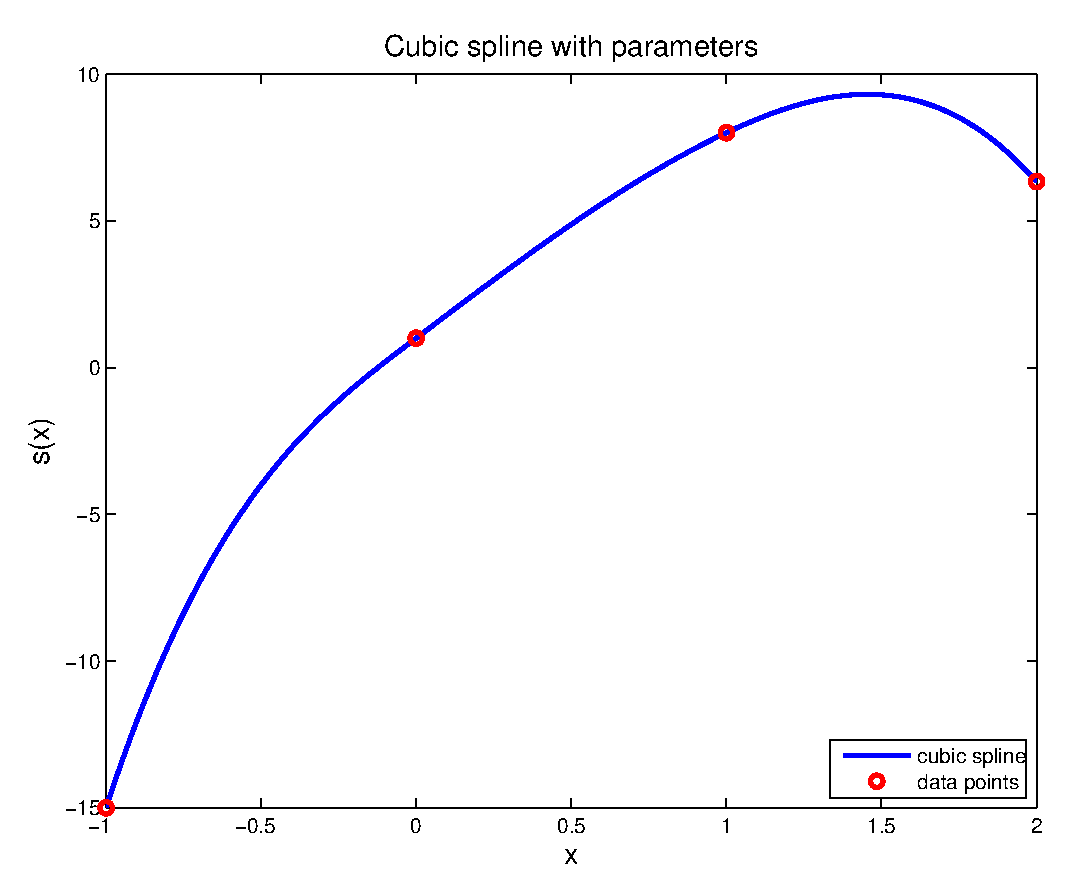
\includegraphics[width=0.5\textwidth]{\problems/ch_piecewisepolynomials/PICTURES/ex_CubicSpline.eps}
\end{center}

\end{solution}
\end{subproblem}
\end{problem}




